% Full instructions available at:
% https://github.com/elauksap/focus-beamertheme

\documentclass{beamer}
\usetheme{focus}

\usepackage[utf8]{inputenc}
\usepackage[T1]{fontenc}
\usepackage[french]{babel}

\usepackage{graphics}
\usepackage{graphicx}

\usepackage{pifont}% http://ctan.org/pkg/pifont
\newcommand{\cmark}{\color{example}\ding{51}}%
\newcommand{\xmark}{\color{red}\ding{55}}%
\newcommand{\fmark}{\ding{229}}%
\newcommand{\itemc}{\item[\cmark]}%
\newcommand{\itemx}{\item[\xmark]}%
\newcommand{\itemf}{\item[\fmark]}%

\usepackage{siunitx}

\title{La fonction alimenter/stocker}
\subtitle{}
\author{ETT - Cours}
\titlegraphic{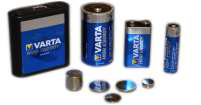
\includegraphics[width=.2\textwidth]{Cours/Premieres/ETT/Seq03_alimenter/S03C01_chaine_energie_alimenter/piles.png}}
\institute{IUT de Cachan}
\date{09 novembre 2018}

\begin{document}
    \begin{frame}
        \maketitle
    \end{frame}
    
    \begin{frame}
        \tableofcontents
    \end{frame}
    
    \section{Généralités}
    \begin{frame}{Définition}
        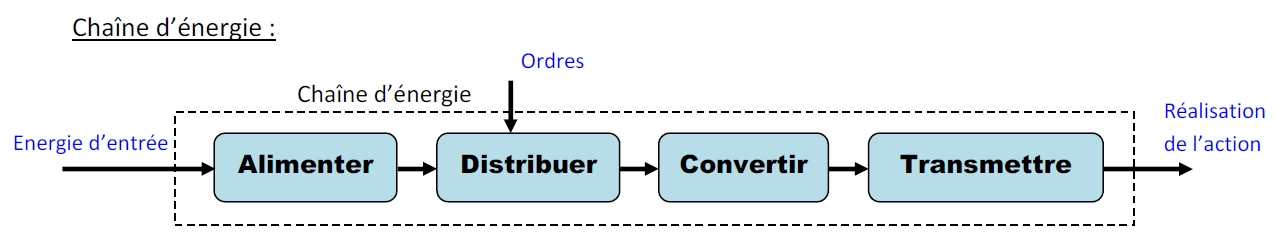
\includegraphics[width=\textwidth]{Cours/Premieres/ETT/Seq03_alimenter/S03C01_chaine_energie_alimenter/images/chaine.jpg}
        \begin{exampleblock}{Définition}
        \visible<2->{Les éléments du bloc \textbf{Alimenter/Stocker} ont pour fonction de fournir l'énergie au système. Cette énergie peut provenir de l'extérieur du système ou être stockée au sein du système.} 
        \end{exampleblock}
    \end{frame}
    
    \begin{frame}{Stocker de l'énergie}
    \begin{block}{Pourquoi stocker de l'énergie ? }
\begin{itemize}
    \item Autonomie 
    \item Décalage temporel
    \item Compensation des fluctuations
\end{itemize}
\end{block}
    \end{frame}
    
    \begin{frame}{Stocker de l'énergie électrique}
        \begin{alertblock}{}
            Il est impossible de stocker de l'énergie sous forme électrique
        \end{alertblock}
        \begin{block}{Stocker sous forme chimique}
            \centering
            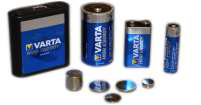
\includegraphics[height=0.2\textheight]{Cours/Premieres/ETT/Seq03_alimenter/S03C01_chaine_energie_alimenter/piles.png}            \begin{description}
                \item<1->[La tension :]{s'exprime en V}
                \item<2->[La capacité] représente la quantité d'électricité stockée dans la batterie.
                Elle s'exprime en \si{Ah}
                \item<3->[La densité énergétique] C’est la quantité d’énergie par unité de masse ou de volume
            \end{description}
        \end{block}
    \end{frame}

    \begin{frame}{Stocker de l'énergie électrique}
        \begin{alertblock}{}
            L'intensité I dans un circuit s'exprime en \si{A}, la capacité (nombre de charges stockées) s'exprime en \si{Ah}.
        \end{alertblock}
        
        \begin{block}{Lien intensité <-> Capacité}
        Une batterie contenant 10Ah sera capable de fournir un courant de 10A pendant 1h, ou encore un courant de 5A
pendant 2h
        \end{block}
    \end{frame}
    
    \begin{frame}{Calculer l'énergie contenue dans une batterie}
        Pour calculer l'énergie présente dans une batterie, il faut multiplier le nombre de charges par la tension. 
        
        \begin{block}{}
        Calculer la quantité d'énergie contenue dans une batterie d'une tension de $U = \SI{3}{V}$, d'une capacité de $Ca=\SI{1.5}{Ah}$.
        \end{block}
        \visible<2->{\begin{exampleblock}{}Une batterie d'une capacité de $C_a= \SI{1.5}{Ah}$ avec une tension de \SI{3}{V} contient une quantité d'énergie $E=U\times C_a = 1.5\times 3$.
        \end{exampleblock}}
    \end{frame}
    
    \begin{frame}{}
        \centering
        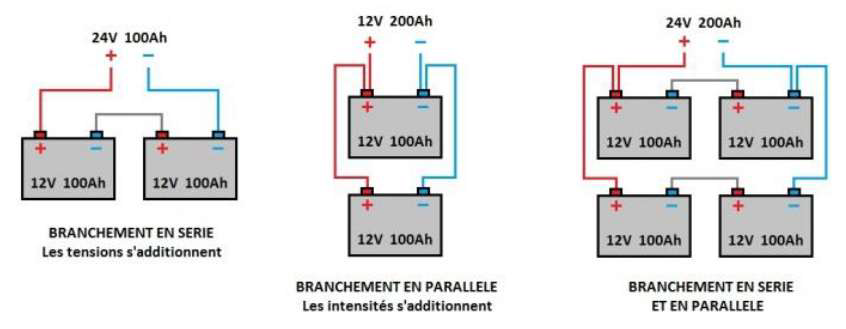
\includegraphics[width=\textwidth]{Cours/Premieres/ETT/Seq03_alimenter/S03C01_chaine_energie_alimenter/images/association.png}
    \end{frame}
    
    \section{Autre forme de stockage}
    
    \begin{frame}{Stocker de l'énergie hydraulique}
        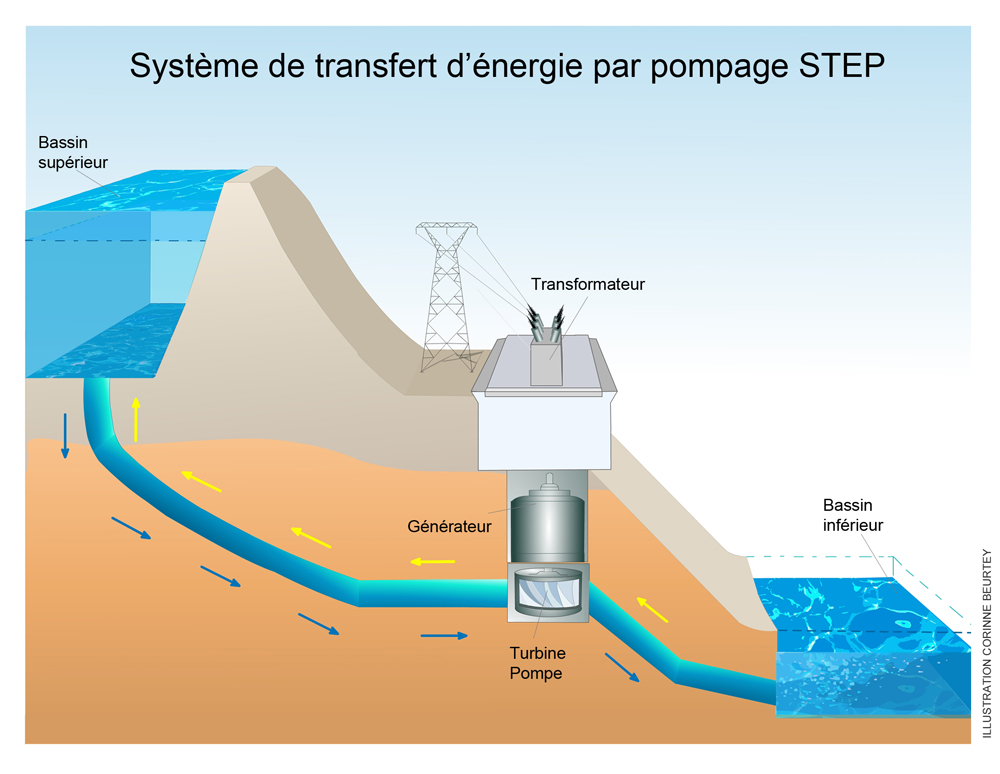
\includegraphics[width=0.7\textwidth]{Cours/Premieres/ETT/Seq03_alimenter/S03C01_chaine_energie_alimenter/images/hydrau.jpg}
    \end{frame}
    
    \section{Les signaux électriques}
    \begin{frame}{Les signaux}
        \begin{block}{définition}
        Un signal est dit périodique si les variations de son amplitude se reproduisent régulièrement au bout d'une période \textbf{T} constante.
        
        \begin{center}
            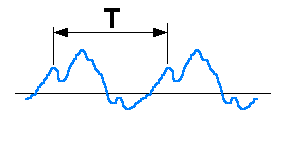
\includegraphics[width=0.5\textwidth]{Cours/Premieres/ETT/Seq03_alimenter/S03C01_chaine_energie_alimenter/images/Signal_periodique.png}
        \end{center}
        \end{block}
    \end{frame}
    
    \begin{frame}{Caractéristiques d'un signal}
        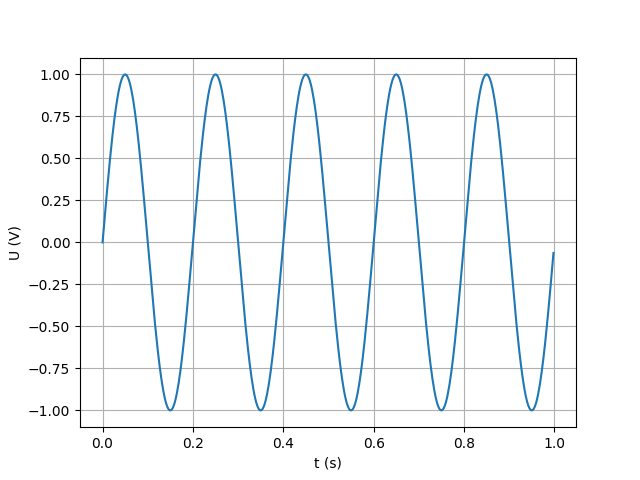
\includegraphics[width=.8\textwidth]{Cours/Premieres/ETT/Seq03_alimenter/S03C01_chaine_energie_alimenter/images/sinus.png}
    \end{frame}
    
    \begin{frame}{Caractéristiques d'un signal}
        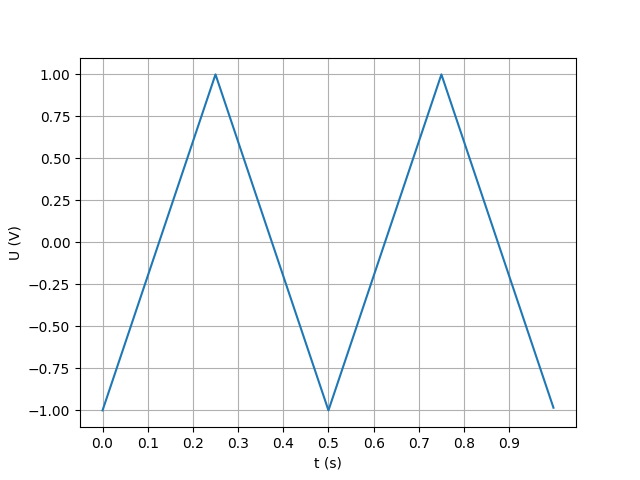
\includegraphics[width=.8\textwidth]{Cours/Premieres/ETT/Seq03_alimenter/S03C01_chaine_energie_alimenter/images/triangle.png}
    \end{frame}
    
    \begin{frame}{Caractéristiques d'un signal}
        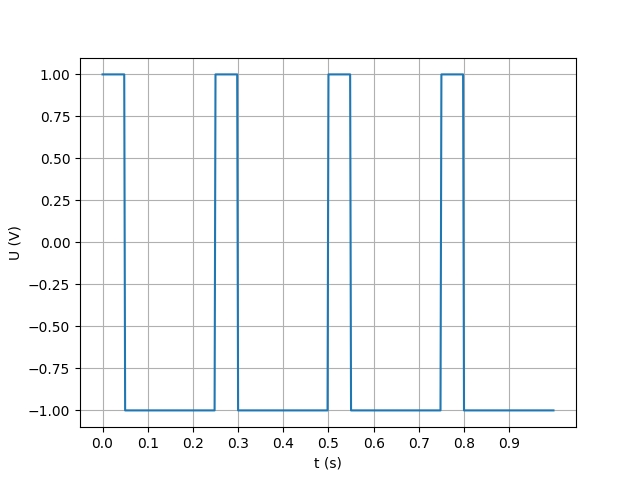
\includegraphics[width=.8\textwidth]{Cours/Premieres/ETT/Seq03_alimenter/S03C01_chaine_energie_alimenter/images/carre.png}
    \end{frame}
    
    \begin{frame}{Branchement d'un appareil de mesures}
        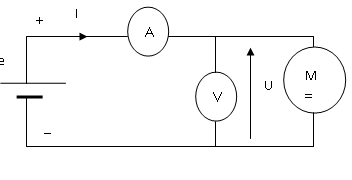
\includegraphics[width=.8\textwidth]{Cours/Premieres/ETT/Seq03_alimenter/S03C01_chaine_energie_alimenter/images/branchement.png}
    \end{frame}
    
    \begin{frame}[focus]
        Questions ? 
    \end{frame}
    
    \appendix
\end{document}
